\chapter{Introduction}
%\addcontentsline{toc}{chapter}{Introduction}
\label{introduction}

%\todolist{
    %Turbulence in the edge and SOL
%}

%---------------------------------------------------------------------------------------------------------------------

The growth of the world's economy is made possible by a continuous increase in primary energy consumption.
%
Indeed, a substantial amount of energy is required in order to keep improving the living standards of both developing and developed economies.
%
As shown in \cref{fig:worldconsumption}, between 1992 and 2017, the primary energy consumption of the world increased by 70\%, from 8 billion to a 13.5 billion tons oil equivalent \citep{Chen2017}.
%
In 2016, the world consumption of energy grew by 1.3\%, and a growth of 2.2\% was recorded in 2017, the highest since 2013.
%
The growth is projected to continue increasing in the next years \citep{BP2017}.
%
Such growth had a direct impact on the climate, particularly through the global emissions of CO$_2$, which doubled in the period 1975-2015 and are projected to triple by 2040 \citep{Chu2017}.
%
The amount of energy generated from fossil fuels needs to be severely limited if the production of greenhouse gases such as CO$_2$ is to be reduced.
%
Therefore, there is an urge to outline possible paths towards sustainable energy production and consumption.
%
In this context, a huge effort is currently devoted to investigate the possibility of using fusion as a source of energy that can ultimately address the increasing world energy demand.

\begin{figure}
    \centering
    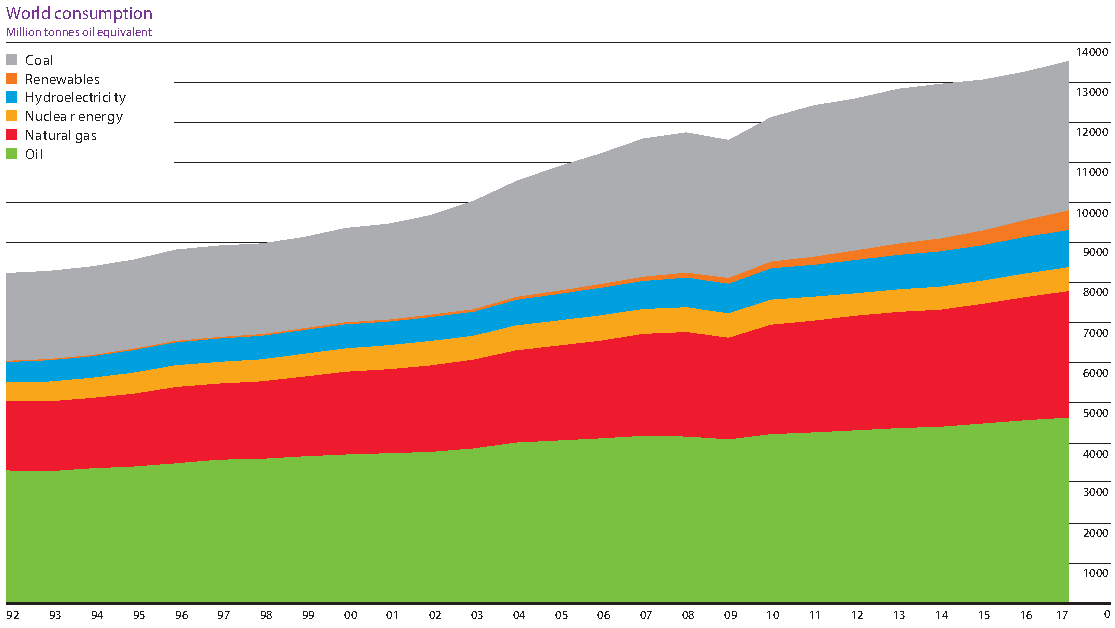
\includegraphics[width=.85\textwidth]{images/2017_world_consumption.pdf}
    \caption{World primary energy consumption between 1992 and 2017 in million tonnes oil equivalent. In 2017 alone, energy consumption grew 2.2\%, with the largest increment provided by natural gas, followed by renewable power and oil. Source: \citet{BP2017}.}
    \label{fig:worldconsumption}
\end{figure}

Fusion is a form of nuclear energy, the main source of energy in the Sun and other stars.
%
Here, light nuclei with combined initial mass $m_i$ recombine into one or more atomic nuclei with mass $m_f$.
%
When $m_f<m_i$, the difference in mass between the initial and final particles is converted into released energy $E$ according to Einstein's relation
%
\begin{equation}
E = (m_i - m_f)c^2,
\label{eq:einstein}
\end{equation}
%
\noindent where $c$ is the speed of light.
%
Among all possible fusion reactions that release energy, the one between deuterium-tritium (DT)
%
\begin{equation}
    ^2_1 \text{D} + ^3_1 \text{T} \rightarrow ^4_2 \text{He}+^1_0\text{n},
\label{eq:dt}
\end{equation}
%
is considered to be the best suited reaction for the first generation of fusion devices \citep{Freidberg2007}.
%
This reaction yields a net energy of $17.6$ MeV that goes into the kinetic energy of the fusion products, approximately $3.5$ MeV to $^4_2 \text{He}$ and 14.1 MeV to $^1_0\text{n}$.
%
The kinetic energy imparted to the neutrons will be used to produce electricity.
%
The energy of the $^4_2 \text{He}$ will be used to heat the fresh fusion fuel and compensate for the unavoidable heat losses, keeping the reaction going.
%
The deuterium for the fusion process can be extracted from sea water.
%
On the other hand, tritium can be obtained from the reaction of the neutron with the lithium in a blanket surrounding the device.
%
A fusion reactor is expected not to produce long-lived radioactive waste.
%
Indeed, with an appropriate choice of materials, half-lives of dozens of years can be achieved \citep{Fetter1988}.

The material in a fusion reactor must be sufficiently well confined with a sufficiently high temperature $T$ and density $n$ for the $^4_2 \text{He}$ energy to balance the energy losses due to radiation, conduction, and convection.
%
This statement can be quantified into a single constraint in terms of $T$, $n$, and confinement time, $\tau$.
%
The confinement time is defined as the energy content of the plasma $W$ divided by the power loss ${P_{\text{loss}}}$, $\tau = {W}/{P_{\text{loss}}}$ (with the thermal energy of the plasma $W$ given by the integral over volume of the energy density $n_a T_a$ summed over all species $a$).
%
Indeed, for self-sustained fusion reactors, the power loss ${P_{\text{loss}}}$ has to be compensated by the energy produced by the fusion reactions, such that $f E_{fp} \ge P_{\text{loss}}$ where $f$ is the number of fusion reactions per time unit and $E_{fp}$ the energy of the charged fusion products.
%
Assuming that the plasma in the reactor is composed by electrons, deuterium, and tritium with roughly the same density and temperature, and assuming that the distribution of energy of the plasma particles follows a Gaussian distribution, a minimum value for the product $n T \tau$ can be found, yielding the condition \citep{Wesson2004}
%
\begin{equation}
    \tau n T > 5 \times 10^{21}\text{~s m$^{-3}$ keV},
\label{eq:lawsoncriteria}
\end{equation}
%
with a minimizing value of $T_{\text{min}}=15$ keV (which is in fact one order of magnitude higher than the temperatures at the sun's core, $\sim 1$ KeV).
%
Equation (\ref{eq:lawsoncriteria}) is commonly known as Lawson's criterion.

At the temperatures necessary for self-sustained fusion, the fusion fuel is fully ionized, i.e., electrons are stripped away from their atomic nuclei as the ionization energy of the plasma elements ($\sim$10 eV) is a few orders of magnitude below the keV range.
%
The resulting neutral gas of dissociated electrons and ions is called a plasma.
%
As both electrons and ions are electrically charged, the particles in the plasma interact through electromagnetic forces.
%
Ultimately, the description of a plasma can be reduced to the understanding of the trajectories of its constituting particles.
%
This usually involves solving an extremely complex set of equations in typically non-trivial geometry settings to study the motion of charged particles in the electromagnetic fields that are both externally applied and generated by the plasma itself.


Several strategies have been devised to confine the plasma in fusion conditions, with two main lines of research pursued today: inertial and magnetic confinement fusion.
%
In inertial confinement fusion, nuclear fusion reactions are initiated through the heating and compression of a fuel target by high-energy laser, electron, or ion beams.
%
With very high plasma densities ($n \sim 10^{30}$ m$^{-3}$), \cref{eq:lawsoncriteria} allows for short confinement times ($\tau \sim 10^{-9}$ s).
%
On the other hand, in magnetic confinement fusion, the plasma is confined by strong magnetic fields.
%
Magnetic confinement fusion reactors are targeted to work at considerably lower densities ($n\sim 10^{20}$ m$^{-3}$) that are, in fact, much lower than the density of air ($n \sim 10^{25}$ m$^{-3}$).
%
This constraints the confinement time to be greater than at least one second, according to \cref{eq:lawsoncriteria}.
%
The present thesis focuses on magnetic confinement fusion.

The magnetic field $\mathbf B=B \mathbf b$ necessary to ensure plasma equilibrium in magnetic fusion devices can be derived from the force balance equation \citep{Freidberg2007}
%
\begin{equation}
    \mathbf J \times \mathbf B = \nabla P,
\label{eq:forcebalanceMHD}
\end{equation}
%
where $\mathbf J$ is the plasma current, related to the magnetic field by Ampère's law
%
\begin{equation}
    \nabla \times \mathbf B = \mu_0 \mathbf J,
\end{equation}
%
and $P$ is the plasma pressure.
%
The force balance equation, \cref{eq:forcebalanceMHD}, is derived from the magnetohydrodynamics (MHD) equation of motion in the steady state limit without flows, and it essentially provides the amount of current necessary to magnetically confine a plasma with finite pressure.
%
From \cref{eq:forcebalanceMHD}, we see that the vectors $\mathbf B$ and $\mathbf J$ should lie on surfaces of constant pressure, as $\mathbf B \cdot \nabla P = \mathbf J \cdot \nabla P = 0$.
%
This statement, combined with the fact that, according to Poincaré's theorem, a compact surface which is everywhere tangential to a non-vanishing vector field free of singularities must have the topology of a torus \citep{Helander2014}, shows that surfaces of constant pressure in a magnetically confined plasma must have a toroidal geometry, and that field lines of $\mathbf B$ and $\mathbf J$ should wind around the torus (see \cref{fig:toroidaldevice}).
%
There are three ways to twist the magnetic field lines around a torus: by driving an electric current through the plasma, by rotating the poloidal cross-section of the magnetic flux surfaces along the toroidal direction, or by making the magnetic axis not lie in a plane (this is called magnetic torsion) \citep{Mercier1964,Helander2014}.
%
Currently, the magnetic confinement fusion device that showed higher confinement times and is more theoretically and experimentally  advanced is the tokamak (\cref{fig:toroidaldevice} a).
%
In tokamaks, magnetic field line twisting is provided by means of a plasma current only.
%
This contrasts with stellarators that usually rely on a combination of both rotation of the flux surfaces' poloidal cross-section and torsion of the magnetic axis.

\begin{figure}
    \centering
    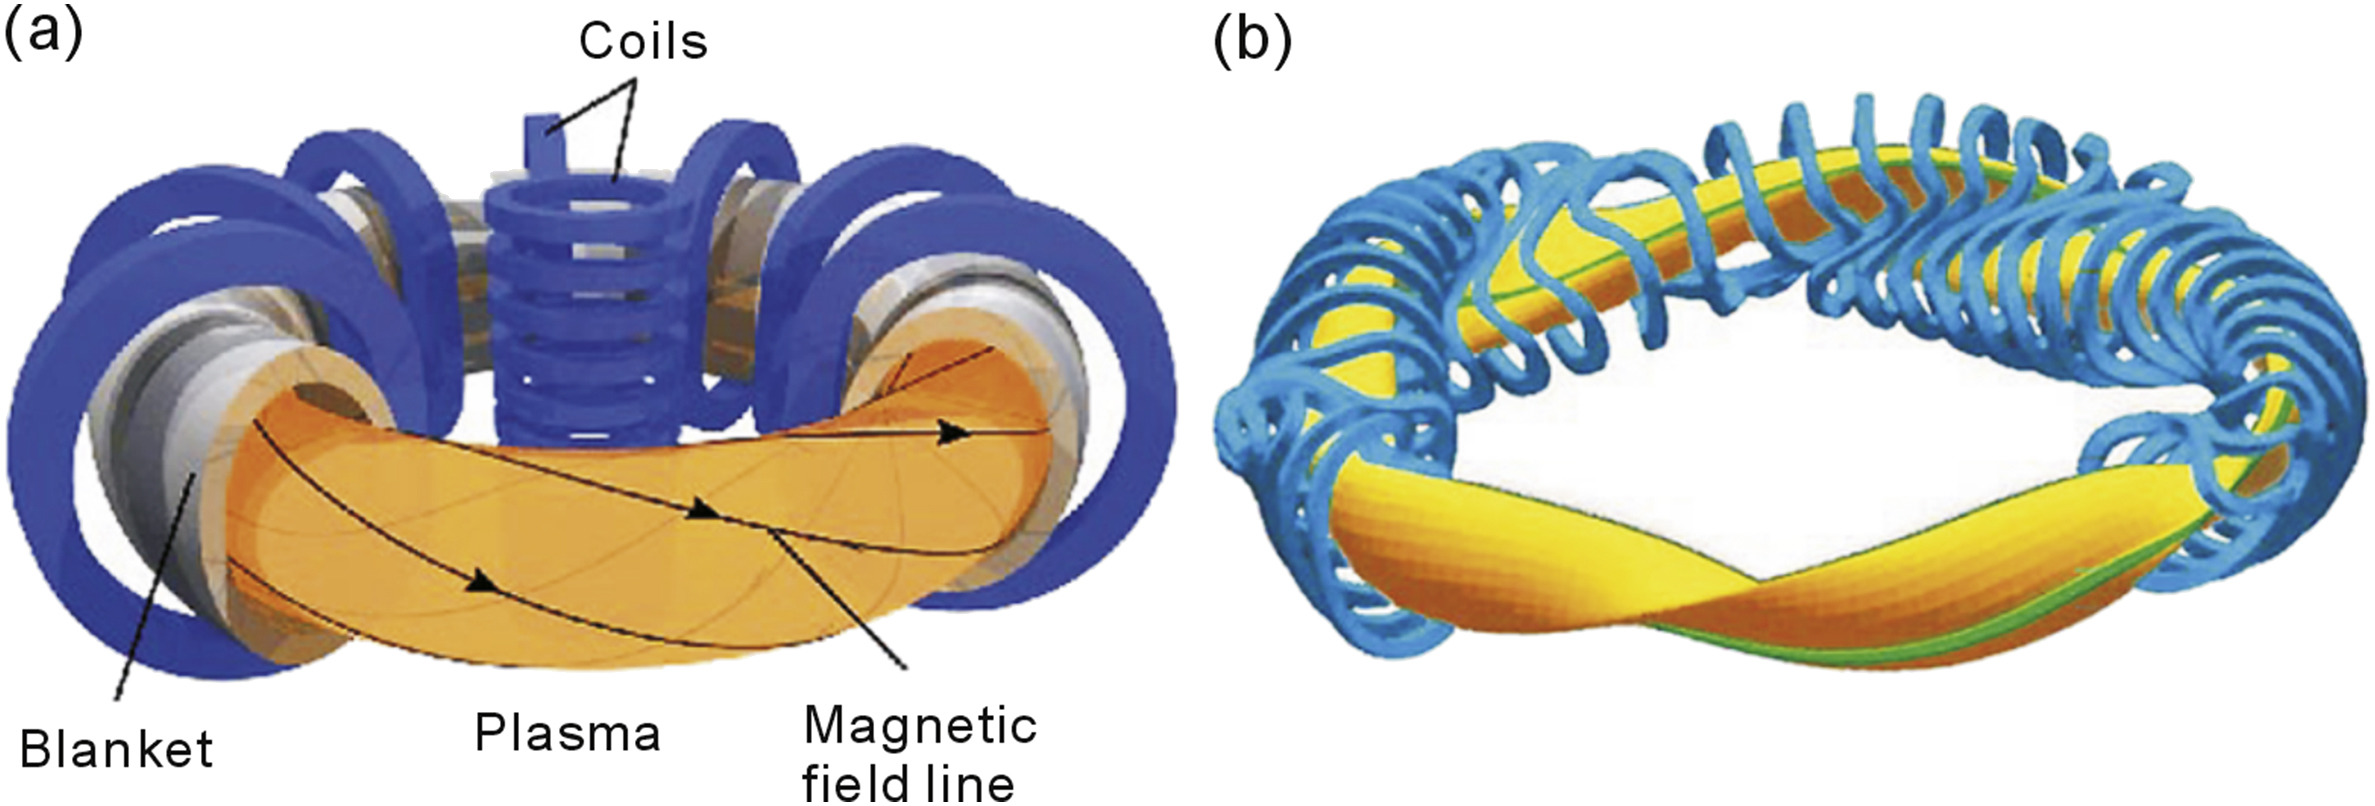
\includegraphics[width=.99\textwidth]{images/tokamak_stellarator.jpg}
    \caption{Schematics of two magnetic confinement fusion designs: tokamaks (a) and stellarators (b). The twist in magnetic field lines in the tokamak is driven by a current generated in the plasma, while in the stellarator, a plasma current is not needed as magnetic field lines are twisted entirely by external non-axisymmetric coils. Source: \citep{Xu2016}.}
    \label{fig:toroidaldevice}
\end{figure}

\section{The Tokamak Device}

In a tokamak, the plasma is confined by means of a magnetic field inside a toroidal chamber, as shown in \cref{fig:toroidaldevice} (a).
%
The largest tokamak in operation today is JET, where the highest ratio $Q$ between the fusion power generated in the reactor and the external heating power, namely $Q \simeq 0.7$, with a triple product $n T \tau \simeq 8 \times 10^{20}$ keV s m${^{-3}}$ was obtained \citep{Jacquinot2010}.
%
The achievements in tokamak research paved the way to the construction of the ITER tokamak in France, expected to produce its first plasma in 2025, with the goal of obtaining $Q=10$ \citep{Aymar2002} and show the feasibility of using magnetic confinement fusion as a  source of energy.
%
A schematic diagram of the ITER fusion reactor is shown in \cref{fig:iter}.
%
\begin{figure}
    \centering
    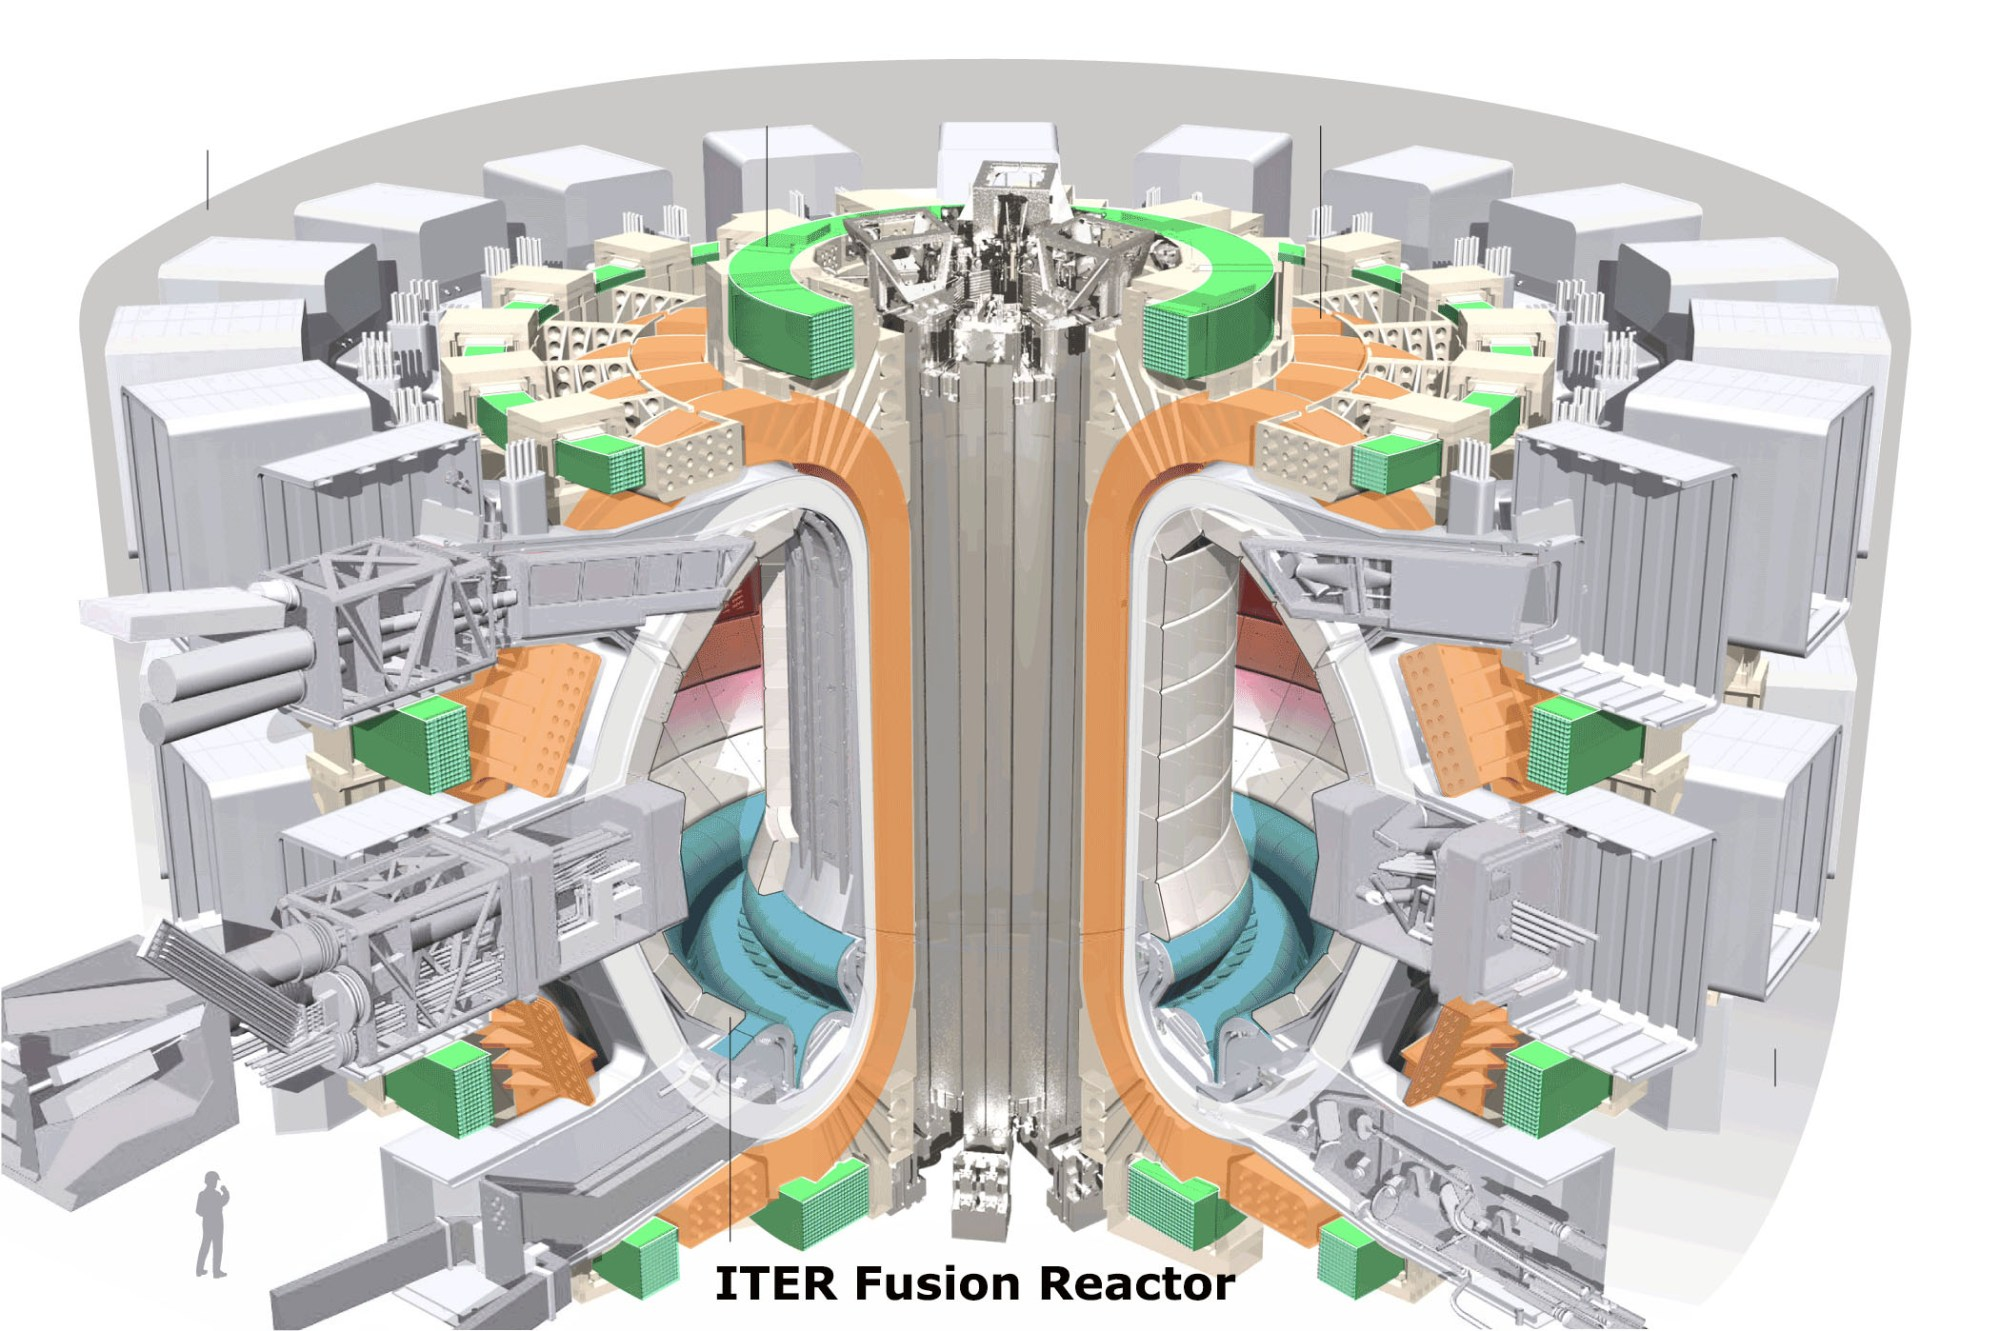
\includegraphics[width=.75\textwidth]{images/iter.jpg}
    \caption{Schematic of the ITER (International Thermonuclear Experimental Reactor) device, including its divertor (blue), external coils (orange and green), and its D-shaped vessel. Source: iter.org}
    \label{fig:iter}
\end{figure}

The magnetic field in a tokamak is generated by a combination of coils arranged on a set of equidistant poloidal planes, creating the toroidal component of the magnetic field, and by plasma current driven by a toroidal electric field which is induced, thanks to a transformer action, by the central coils in \cref{fig:toroidaldevice} (a).
%
The plasma in the tokamak can be heated to temperatures of a few keV leveraging the fact that plasma current produces ohmic heating.
%
However, temperatures above 10 keV are necessary to ignite the fusion reactions are achieved by means of additional heating using particle beams or electromagnetic waves \citep{Wesson2004}.
%
While such temperatures are expected to be achieved in the plasma core, the periphery region of the plasma should be substantially colder in order not to damage plasma-facing materials, ensuring a reasonable lifetime of the device, and avoiding the impurities sputtered by the solid walls to contaminate the plasma and decrease its stability and confinement properties.
%
Ultimately, the complex interaction between the plasma and the device can constitute a limiting factor in achieving Lawson's criterion, \cref{eq:lawsoncriteria}.
%
For this reason, several mechanisms to control the plasma-solid interaction are devised.
%
In most of present tokamaks and in ITER, the flux of heat and particles is typically diverted to the bottom of the device in the divertor region (blue region in \cref{fig:iter}).
%
A divertor configuration of a tokamak plasma is shown in \cref{fig:plasmaboundary}, together with a typical structure of the magnetic flux surfaces that allow the removal of heat and particles through the divertor.
%
In this thesis, we mainly focus on the plasma periphery region, composed of the edge, where the magnetic field lines lie on flux surfaces that do not intercept the wall of the device, and the scrape-off layer (SOL), where the magnetic field lines intercept the wall of the device (see \cref{fig:plasmaboundary}).
%
The magnetic flux surface that defines the separation between these two regions is called the last closed flux surface, or separatrix.
%
\begin{figure}
    \centering
    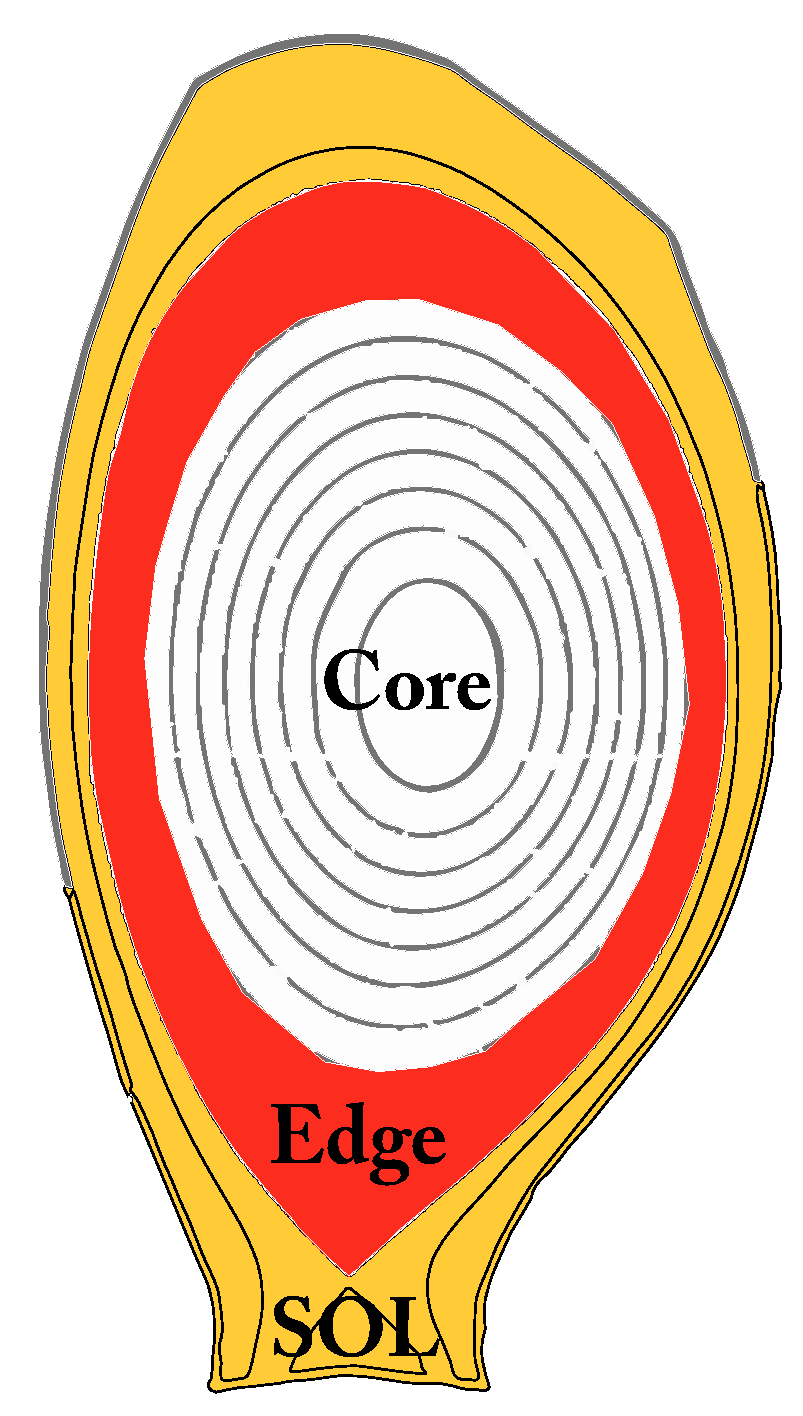
\includegraphics[width=.35\textwidth]{images/Core_Edge_Sol.pdf}
    \caption{Poloidal cross-section of a tokamak plasma, divided into three regions: most inward hotter region (core), most outward region with closed magnetic flux surfaces in red (edge), region with magnetic field lines that intercept the wall of the device in yellow (SOL).}
    \label{fig:plasmaboundary}
\end{figure}

\section{Modelling of Plasma Dynamics at the Tokamak Periphery}
\label{sec:plasmamodelling}

A full understanding of the dynamics at the tokamak edge and SOL regions is essential for the successful operation of future fusion experiments and reactors, as this region is responsible for much of the overall confinement of the tokamak device \citep{Ricci2015}.
%
In the edge region of magnetic fusion devices operating a regime of improved confinement (the so-called H-mode observed in many present devices and predicted to occur in many future devices such as ITER) a pedestal develops, i.e., the profiles of density and temperature become very steep near the separatrix and a radial electric field is formed, which is thought to be responsible for the reduction of turbulence levels \citep{Wagner1984}.
%
The H-mode pedestal can be periodically relaxed due to Edge-Localized Modes (the so-called ELMs), yielding large amplitude bursts of particle and heat exhaust into the SOL \citep{Leonard2014}, which are a major concern on the way to fusion.
%
The SOL region, on the other hand, controls the plasma heat exhaust, plasma refuelling and the removal of fusion ashes, and sets the boundary between the plasma and the vessel.
%
Moreover, in the SOL, due to the presence of a complex magnetic geometry, typical coordinate systems used for core simulations are found to be singular.
%
Due to the crucial role of the tokamak periphery region on the performance of a fusion device, significant experimental and theoretical work has been devoted in the last few decades to the understanding of the fundamental mechanisms governing the dynamics of this region \citep{Loarte2007}.

The dynamics of the plasma at the tokamak periphery region is observed to be strongly nonlinear. Fluctuations occur on a broadband range of wavenumbers $\mathbf k\sim \nabla \log n \sim \nabla \log T$ and frequencies $\omega\sim |\partial_t \log n|\sim|\partial_t \log T|$ \citep{Scott2007}, and are strongly anisotropic, i.e., wavenumbers parallel to the magnetic field ($k_\parallel = \mathbf k \cdot \mathbf b$) are much smaller than the perpendicular ones ($\mathbf k_\perp=\mathbf k - k_\parallel \mathbf b$).
%
Modes present in the edge can have perpendicular wavelengths as low as the ion gyration radius $\rho_i$ ($\rho_i\sim 0.3$ cm at $T=1$ keV an $B=1$ T) and, in the SOL, the dominant turbulent modes have a perpendicular wavelengths that are usually one order of magnitude or more smaller than $\rho_i$ ($\rho_i\sim 0.3$ mm at $T=10$ eV an $B=1$ T) \citep{Agostini2011}.
%
The typical $\rho_i$ lengths at the tokamak periphery and core are indeed much smaller than the tokamak minor and major radius, $a$ and $R$, respectively, of typical magnetic field gradient lengths $L_B \sim R$, and of typical scale lengths of the fluctuations in the parallel direction $L_\parallel \sim 1/k_\parallel$.
%
Regarding turbulent frequencies $\omega$, these are typically much lower than the ion gyrofrequency $\Omega_i$ \citep{Hahm2009}.

The gyrokinetic model is the most established one to describe tokamak turbulence in the ordering $k_\perp \rho_i \sim 1$, $\omega/\Omega_i \ll 1$ and $k_\parallel/k_\perp \ll 1$ \citep{Catto1978a,Frieman1982,Brizard2007a,Parra2008,Hahm2009}.
%
Gyrokinetic theory provides a rigorous framework to remove the details of the charged particle's gyromotion and other high frequency phenomena.
%
A variety of numerical methods have been developed to solve numerically the gyrokinetic equation, with the two main types being the continuum \citep{Jenko2001} and the particle-in-cell \citep{Lee1987} methods.
%
These methods have allowed major progress in the understanding of tokamak turbulence in the core, where a low collisionality model can be used and plasma quantities can be split between fluctuating and time-averaged components, in order to evolve only the former (the so-called $\delta f$ approach) \citep{Kinsey2011}.
%
Among several gyrokinetic codes used to describe plasma turbulence in the tokamak core, we mention CGYRO \citep{Candy2016}, GEM \citep{Parker1999}, GENE \citep{Jenko2000a,Gorler2011}, GKV \citep{Watanabe2006}, GKW \citep{Peeters2009}, GS2 \citep{Kotschenreuther1995,Dorland2000a}, GYRO \citep{Candy2003}, GYSELA \citep{Latu2007}, and ORB5 \citep{Jolliet2007}.
%
However, some complications arise when applying established gyrokinetic simulations for the tokamak core to the plasma periphery.
%
In the edge and SOL, the plasma is turbulent, with fluctuation levels of order unity, which renders conventional $\delta f$ gyrokinetic approaches unable to handle such conditions, as opposed to more computational demanding approaches that do not separate fluctuating and time-averaged quantities, also called full-F approaches.
%
Furthermore, while the core is weakly collisional with temperatures of $\sim 10$ keV, the tokamak periphery is characterized by temperatures ranging from the keV range at the inner edge to a few eV in the far SOL region, with a similar order of magnitude variation for the plasma density.
%
The development of a gyrokinetic collision operator derived from first principles, able to handle arbitrary collisionality regimes in a turbulent setting is still the subject of ongoing research \citep{Hirvijoki2017}.
%
Indeed, there are only a few recent attempts to use gyrokinetic simulations for the tokamak periphery.
%
Among these, we mention COGENT \citep{Dorf2013}, ELMFIRE \citep{Heikkinen2008}, G5D \citep{Kawai2017}, GKEYLL \citep{Shi2017}, TEMPEST \citep{Xu2010a}, and XGC1 \citep{Chang2009}.

We remark that the effect of Coulomb collisions between charged particles is crucial to accurately predict the growth rate of instabilities occurring in magnetic confinement fusion devices and to predict the level of turbulent transport \citep{Barnes2009}.
%
Collisions are not only a major regulator of low-frequency turbulence and associated transport, but they also determine the steady state of the system by dictating the long term evolution of the plasma quantities.
%
Although several theoretical studies have emerged in order to derive an appropriate Coulomb collision operator for drift-kinetic and gyrokinetic formulations \citep{Brizard2004,Sugama2015,Burby2015}, such operators still involve a complicated nonlinear six-dimensional phase-space integral to be performed \citep{Hirvijoki2017}.
%
Due to constraints related to code parallelization and computational resources, a numerical implementation of such intricate formulations of the Coulomb collision operator is still out of reach.

Because of the limitation of current gyrokinetic models, for numerical reasons, and due to their simplicity, fluid models that incorporate the drift ordering approximation $k_\perp \rho_i \ll 1$ have become the standard for SOL theoretical and numerical modelling \citep{Zeiler1997,Ribeiro2008a}.
%
Notable examples include BOUT++ \citep{Dudson2009}, GBS \citep{Ricci2012a}, GDB \citep{Zhu2018}, GRILLIX \citep{Stegmeir2018} HESEL \citep{Nielsen2015}, STORM \citep{Easy2014}, and TOKAM3X \citep{Tamain2009}.
%
Such models are usually derived from the Braginskii fluid equations \citep{Braginskii1965}, where the plasma is assumed to be close to thermodynamic equilibrium because of collisions, i.e., assuming that the electron $\nu_e$ and ion $\nu_i$ collision frequencies are larger than the typical turbulent frequencies.
%
For L-mode cold SOL plasmas, fluid models have been successfully benchmarked against experimental results \citep{Riva2016,Militello2016}.
%
Moreover, in such regimes, previous studies on the plasma dynamics at the SOL region \citep{Ricci2013, Mosetto2015} have estimated key SOL parameters such as cross-field transport, plasma scale lengths, and instability thresholds through a careful combination of linear analysis of the turbulent modes and turbulent saturation mechanisms, yielding a simple physical picture of SOL turbulence as the interplay between turbulent transport and plasma losses at the vessel wall.
%
However, inside the separatrix, in the edge region, although turbulence is still mediated by low-frequency fluctuations, the plasma becomes hotter, less collisional, and small scale $k_\perp \rho_i \sim 1$ fluctuations become important \citep{Hahm2009}.
%
Also, when events such as ELMs expel large amounts of heat and particles to the SOL and to the wall, the description of such high-temperature structures requires a kinetic treatment valid at arbitrary collision frequencies, such as drift-kinetic theory \citep{Hazeltine2003}.
%
These ultimately require to incorporate the effects of Coulomb collisions using an accurate Coulomb collision operator.

We believe that a model that evolves a set of three-dimensional moments of the kinetic distribution function represents the best choice to simulate tokamak periphery plasmas in an accurate and efficient manner.
%
Such a framework has the inherent flexibility of providing a description that spans from the fluid models, when a low number of moments is used and a coarse plasma description is needed, to fully kinetic models, for accurate plasma simulations.
%
To build this model, the plasma distribution function $f$ is expanded in a suitable set of basis functions, i.e., a set of orthogonal polynomials ensuring that the expansion coefficients converge rapidly in order to allow manageable numerical implementation and simulations with a minimum number of terms.
%
In this work, we show that this model, which is indeed a moment-hierarchy, formulated in terms of Hermite and Laguerre orthogonal polynomials, fulfills these requirements, and that it can be used to study the dynamics at the tokamak periphery, both in the fluid and in the gyrokinetic regime.
%
The use of Hermite polynomials in plasma physics can be traced back to the work of \citet{Grad1963}, which used a tensorial formulation of the Hermite polynomials, the so-called reducible Hermite polynomials [as opposed to the irreducible ones used in \citet{Balescu1988}].
%
In fact, the orthogonal basis associated with a Gaussian weight consists of Hermite polynomials.
%
The Gaussian function is relevant for statistical and plasma physics as the long term and stationary solution of the collisional kinetic equation is given by the Maxwell-Boltzmann distribution (a Gaussian function in velocity space) \citep{Helander2002}.
%
We note that, although moment-hierarchy methods have a long history in plasma physics \citep{Grad1963,Braginskii1965,Balescu1988}, only recently such formulations were developed for arbitrary collisionality regimes, using reducible \citep{Hirvijoki2016}, irreducible \citep{Ji2009}, and scalar \citep{Jorge2017} Hermite polynomials.

\section{Scope and Outline of the Thesis}

With the final goal of gaining a deeper understanding and obtaining a predictive tool for the plasma dynamics in the periphery region of magnetic confinement fusion devices, in the present thesis, we develop a moment-hierarchy framework able to evolve the plasma dynamics at the tokamak periphery.
%
A first-principles model is developed based on the careful reconstruction of the motion of single charged particles in a regime relevant for the tokamak periphery.
%
We consider first the drift-kinetic limit assuming $k_\perp \rho_i \ll 1$, a regime of interest for the SOL.
%
Then, gyrokinetic fluctuations at $k_\perp \rho_i \sim 1$ are included.
%
The collective motion of particles is described by an appropriate kinetic equation, including the effect of Coulomb collisions.
%
Aiming for a numerical efficient framework, we expand the distribution function in  a Hermite-Laguerre moment-hierarchy set of equations valid at arbitrary collisionalities, where the integro-differential character of the Coulomb collision operator is converted into linear combinations of moments of the distribution function.
%
The feasibility  of the numerical implementation is shown by the study of the linear evolution of electron-plasma waves and of the drift-wave instability.
%
This study serves not only as a proof of concept of the Hermite-Laguerre formulation, but it also allows, for the first time, the accurate calculation of the impact of collisions in such linearized systems at arbitrary collisionalities.

We note that, in the present work, we focus on the electrostatic limit, which requires three criteria to be satisfied: (1) that $\beta=n T_e/(B^2/2\mu_0) \ll 1$, (2) that $\alpha = \beta a/L_p$ stays below the electromagnetic ballooning instability threshold, and (3) that the frequency of interest is far below the shear Alfvén frequency.
%
While condition (1) is, in general, valid across the tokamak periphery region, condition (2) can be broken down in the edge region in the H-mode regime and condition (3) may be violated near an X-point where parallel wavenumbers can make the shear Alfvén frequency similar to the one of the turbulence.
%
Therefore, we note that the electrostatic approximation employed in this work rules out drift-Alfvén coupling and the treatment of peeling-ballooning modes in the edge.
%
An extension of the model derived here to include electromagnetic perturbations will be addressed in a future publication \citep{Frei2019}.
%
Finally, we point out that the Coulomb collision operator and its velocity moments derived in this work remain unchanged when electromagnetic perturbations are taken into account.

This thesis is structured as follows.
%
In \cref{ch:dk}, we develop a full-F drift-kinetic model to describe the plasma dynamics in the scrape-off layer region of tokamak devices at arbitrary collisionalities, closely following \citep{Jorge2017}.
%
The formulation is based on a gyroaveraged Lagrangian description of the charged particle motion, and the corresponding drift-kinetic Boltzmann equation that includes a full Coulomb collision operator.
%
The Hermite–Laguerre velocity space decomposition of the distribution function is used, and a set of equations to evolve the coefficients of the expansion is presented, including the moments of the Coulomb collision operator, therefore describing plasma distribution functions arbitrarily far from equilibrium.
%
A fluid closure in the high collisionality limit is presented, and the corresponding fluid equations are compared with previously derived fluid models.

In \cref{ch:gk}, a gyrokinetic moment-hierarchy model describing the plasma dynamics in the tokamak periphery is derived within a full-F framework.
%
With respect to the drift-kinetic model of \cref{ch:dk}, this model evolves periphery turbulence in the presence of time-dependent electrostatic fluctuations on scale lengths ranging from the ion gyroradius to typical time-averaged gradient lengths.
%
The formulation is based on a nonlinear second order accurate gyrokinetic equation, derived from Hamiltonian perturbation theory methods.
%
The electrostatic field is evolved according to the gyrokinetic Poisson's equations.
%
A moment-hierarchy formulation of the resulting set of equations is performed, yielding a fluid-like set of equations, valid at $k_\perp \rho_i \sim 1$.

A moment expansion of the Coulomb collision operator valid at arbitrary collisionality and $k_\perp \rho_i \sim 1$ is presented in \cref{ch:op}.
%
This is done by performing a multipole expansion of the Rosenbluth potentials, similar to commonly employed multipole expansions in electrostatics \citep{Jackson1999}.
%
This allows us to derive the dependence of the full Coulomb collision operator on the particle gyroangle in terms of scalar spherical harmonics.
%
Finally, the resulting operator is projected onto a Hermite-Laguerre polynomial basis, yielding analytically closed formulas for numerically implementation.

In \cref{ch:epw}, following \citep{Jorge2018a}, the linearized moment-hierarchy equation is numerically solved to describe the dynamics of electron-plasma waves.
%
The damping rate, frequency and eigenmode spectrum of electron-plasma waves are found as a function of the collision frequency and wavelength.
%
A comparison is made with the collisionless limit and with simplified collision operators, where large deviations are found in the damping rates and eigenmode spectra.
%
Furthermore, we show the presence of a purely damped entropy mode, characteristic of a plasma where Coulomb collisions are dominant.
%
The dispersion relation of this mode is analytically derived and compared with numerical results.

In \cref{ch:dwi}, we focus on the drift-wave instability.
%
We show that the moment-hierarchy framework allows retrieving established collisional and collisionless limits, closely following \citep{Jorge2018}.
%
At the intermediate collisionalities relevant for present and future magnetic nuclear fusion devices, deviations with respect to collision operators used in state-of-the-art turbulence simulation codes show the need for retaining the full Coulomb operator in order to obtain both the correct instability growth rate and eigenmode spectrum.
%
We note that, ultimately, this may significantly impact quantitative predictions of transport levels.

Finally, in \cref{ch:conclusion}, the results and outlook of the thesis are summarized.